% last updated in April 2002 by Antje Endemann
% Based on CVPR 07 and LNCS, with modifications by DAF, AZ and elle, 2008 and AA, 2010, and CC, 2011; TT, 2014

\documentclass[runningheads]{llncs}
\usepackage{graphicx}
\usepackage{amsmath,amssymb} % define this before the line numbering.
\usepackage{ruler}
\usepackage{color}
\usepackage{array}
\usepackage{float}
\usepackage{subfig,caption}
%\usepackage{subcaption}
\usepackage{comment}
\renewcommand{\arraystretch}{1.1}
\usepackage[width=122mm,left=12mm,paperwidth=146mm,height=193mm,top=12mm,paperheight=217mm]{geometry}
\begin{document}
% \renewcommand\thelinenumber{\color[rgb]{0.2,0.5,0.8}\normalfont\sffamily\scriptsize\arabic{linenumber}\color[rgb]{0,0,0}}
% \renewcommand\makeLineNumber {\hss\thelinenumber\ \hspace{6mm} \rlap{\hskip\textwidth\ \hspace{6.5mm}\thelinenumber}}
% \linenumbers
\pagestyle{headings}
\mainmatter
\def\ECCV14SubNumber{***}  % Insert your submission number here

\title{Analyzing The Performance of Multilayer Neural Networks for Object Recognition} % Replace with your title

\titlerunning{ECCV-14 submission ID \ECCV14SubNumber}

\authorrunning{ECCV-14 submission ID \ECCV14SubNumber}

\author{Anonymous ECCV submission}
\institute{Paper ID \ECCV14SubNumber}


\maketitle

\begin{abstract}

\end{abstract}


\section{Introduction}
The break-through work of \cite{Kriz} created a big splash in the computer vision community by presenting a convolutional neural network model which easily surpassed all existing methods on the Imagenet ILSVRC-2012 challenge.  The top-5 error rates dropped by an exceptional amount to 16.4\% from  26.2 \% (achieved by the second best alternative.) At that time, it was unclear if these networks would be useful for other computer vision tasks. The recent work of \cite{Decaf} demonstrated that features learnt by such massive networks generalize and achieve state of the art results on classification datasets such as SUN-397, Caltech-UCSD Birds and Caltech-101 among others. 

In a more recent big development (R-CNN)\cite{Rcnn}, features extracted using convolutional networks were succesfully used to achieve results on object detection which dwarf the existing state of art by a big margin. They achieved a mAP of 54.1 (as compared to 41.7 in  \cite{regionlets}) on PASCAL VOC 2007 detection challenge and showed impressive results on the task of semantic segmentation. The significance of these results can be well appreciated in light of the fact that negligible progress was made over the last few iterations of the PASCAL-VOC challenge. These observations strongly suggest that we might be on the brink of a feature revolution akin to the one ushered by introduction of HOG \cite{Hog} and SIFT \cite{Sift} in the mid 2000's.  

It is not the first time that convolutional neural networks (CNNs) have generated a great interest in the computer vision community. In late 80s and early nineties LeNets \cite{Lecun89} achieved state of art performance on the task of MNIST digit classification. By the end of nineties and throughout the last decade interest in neural networks waned and they were attributed as dark art. One of the main reasons behind this was the fact that a large number of parameters such as the number of layers, number of units in each layer, the learning rate needed to be manually set in order to succesfully train these networks. Support Vector machines on the other hand provided an easy alternative for achieving the same performance levels with only one parameter (C) to tune. However, given the impressive performance of CNN's - the stage is all set for their second renaissance in mainstream computer vision. 

In this work we take the view that rich feature heirarchies provided by convolutional nets are an interesting object which are very likely to emerge as the prominent feature extractor for computer vision models over the next few years. Feature extractors such as SIFT and HOG afford an intuitive interpretation of templates composed of oriented edge filters. However, currently we have little understanding of what different layers of a deep convolutional network encode and what is the most efficient way of using this information. We believe that developing such an understanding is not only an interesting scientific pursuit but is also the stepping stone towards designing methods which can optimally use these features.  

This paper is focussed on a scientific investigation of multilayer convolutional neural networks and presents insights which would be useful towards developing an object recognition system. We carry out this investigation by asking four questions detailed below.

For a long time proponets of multilayer networks have argued that unsupervised pre-training followed by finetuning is helpful for improving performance on discriminative tasks such as image classification \cite{GoogleCat}, \cite{DeepPre}, \cite{HintonPre}. However recent work of \cite{Decaf} and \cite{Rcnn} have made a strong case for the utility of learning features using discriminative pretraining and finetuning them for a specific task at hand. This leads us to our first question,
\begin{center}
\textit{``What happens during finetuning of a discriminatively pretrained network?"}
\end{center}
Most of the popular computer vision models can be categorized either as a Bag of Words model or as a template based model. We would like to understand if the features from the conv-net could be interpreted in any of these ways. More concretely we wish to understand, 
\begin{center}
\textit{``Is there information in the location of where filter activate or is it the magnitude of their activation?"}
\end{center}

Existence of Grand-Mother cells (units tuned to a very specific visual entity)  has been a hotly debated topic in neuroscience \cite{Grandmother} and has been fairly discussed in papers such as \cite{GoogleCat} proposing multilayer architectures for object recognition. We explore this question in the form of: 
\begin{center}
\textit{``Does a multilayer CNN contain Grand-Mother Cells? Or, in other words, how distributed is the learned representation?" }
\end{center}
The last and the final question we address is,
\begin{center}
\textit{``How does the training of CNN progress over time? Do we really need 7 days?"}
\end{center}

The rest of the paper describes the answer to these four questions and is organized as following: section \ref{sec:train} details the procedure used to train conv-nets.  Sections \ref{sec:fine} \ref{sec-where-info} \ref{sec:grand-mother}\ref{sec:speed} are devoted to the four questions and our analysis is concluded in \ref{sec:concl}.
\section{Training Procedure}
\label{sec:train}
\subsection{Network-Architecture and Nomenclature}
\label{sub:net-arch}
For all our experiments we closely follow the architecture proposed in \cite{Kriz}. The first 2 layers consist of 4 sublayers each - convolution (conv), followed by rectified linear units (relu), pooling (pool) and contrast normalization (norm). Layers 3, 4 are composed of convolutional units followed by relu units. Layer 5 consists of convolutional units, followed by relu and pooling. The last two layers are fully connected (fc). In this work when we refer to a layer without referring to a particular sub-layer - then for layer 1,2,5 we mean the output of the pooling stage and for layers 3,4,6,7 we mean the output of relu units. We trained all our models using the publically available code \cite{caffe} and Nvidia K40 GPUs. Our imagenet network was trained for 310000 iterations and achieves an error rate only about 2\% higher on the ILSVRC validation set 2012. \newline
We use the term Alex-Net to refer to a CNN trained using the architecture described above. FT (ft) or FT-Net refers to a finetuned network whereas as FC-FT(fc-ft) or FC-FT-Net refers to a network finetuned by setting the learning rate of convolutional layers to zero. We use the terms CNNs and conv-nets synonymously to refer to Alex-Net kind of multilayer network architectures. Terms filter/unit are used interchangeably to refer to filters of the CNN and GT-BBOX/gt-bbox stands for Ground truth bounding boxes from the PASCAL-VOC-2007 detection challenge and mAP refers to mean average precision \cite{Pascal}.

\subsection{Training Setup} 
\label{sub:train-setup}
  Unless otherwise specified all our results for image and gt-bbox classification are obtained by training on linear SVM's on train-val sets of PASCAL-VOC-2007 \cite{Pascal} challenge and tested on the test set. For detection we closely follow the R-CNN approach described in \cite{Rcnn}. \newline
For our experiments with the SUN-397 \cite{sun} dataset we use a non-standard train-test split since it is infeasible to finetune conv-nets for 10 different subsets as proposed in \cite{sun}. In particular we randomly split the dataset into 3 parts namely train-val-test using 50\%,10\% and 40\%. The distribution of classes is uniform across all the 3 sets. We only use these results to support our investigations and not to compare with other scene-classification methods.  
 
\subsubsection{Fine-Tuning}
\label{sub:fine-train}
For a particular task, we fine-tune conv-nets by running SGD (Stochastic Gradient) with a starting learning rate set to $\frac{1}{10}^{th}$ of the intial learning rate of the imagenet model. This choice has been made because we donot want to drastically change the parameters of the network and overfit to the training set. At every 20,000 iterations we reduce the learning rate by a factor of 10 and use a mini-batch size of 128. In order to finetune our networks for PASCAL-VOC-2007 detection setting we use region proposals for training closely following the procedure described in \cite{Rcnn}. Unless otherwise stated, the finetuned network for PASCAL experiments is finetuned for 70K iterations whereas that for SUN is finetuned for 40K iterations.

\section{What happens when a discriminatively pretrained network is finetuned?}
\label{sec:fine}
Finetuning a network is the process of slowly updating pre-learned parameters to minimize a target loss function for a new task at hand. Since, convolutional networks have a large number of parameters they are prone to overfitting when trained on small datasets. Finetuning can be considered as a method of transfer learning and recent results from \cite{Rcnn}\cite{Decaf} present a strong case that this methodology boosts performance. Although, unsupervised pretraining has widely studied in the multilayer network literatue \cite{HintonPre}\cite{DeepPre}, till date, there has been almost no work analysing the effect of fine-tuning on different layers of a discriminatively trained multilayer convolutional networks such as the Alex-Net.

We start our analysis by investigating how the entropy of filters across different layers changes as a result of discriminative fine-tuning (see sec \ref{sub:fine-entropy}). Since, entropy of a filter can be evaluated at different threshold level of activations we propose the metric of Area under the Entropy curve (AuE) to judge changes in filter selectivity. Our main finding is that most of the learning during finetuning happens only in the top two fully connected layers. Motivated by this observation, we finetune networks for PASCAL detection and SUN-397 scene classification task by setting non-zero learning rates only in the top 2 layers (see sec\ref{sub:fine-fc-only}). We find this results in a negligible drop in performance and allows for moderate speedups in finetuning time. Other conclusions are presented in the sec \ref{sub:fine-discussion}.

\subsection{Entropy Analysis}
\label{sub:fine-entropy}
We compute entropy of each filter for all layers of Alex-Net and FT-Net using the ground-truth bounding boxes from the VOC-2007 test-set as input to these networks. For each filter, we collect all activations in response to ground truth bounding boxes. Next, we sort the scores in decreasing order and compute entropy of the distribution of 20 PASCAL classes at 100 equally spaced thresholds.

\begin{figure}
\centering
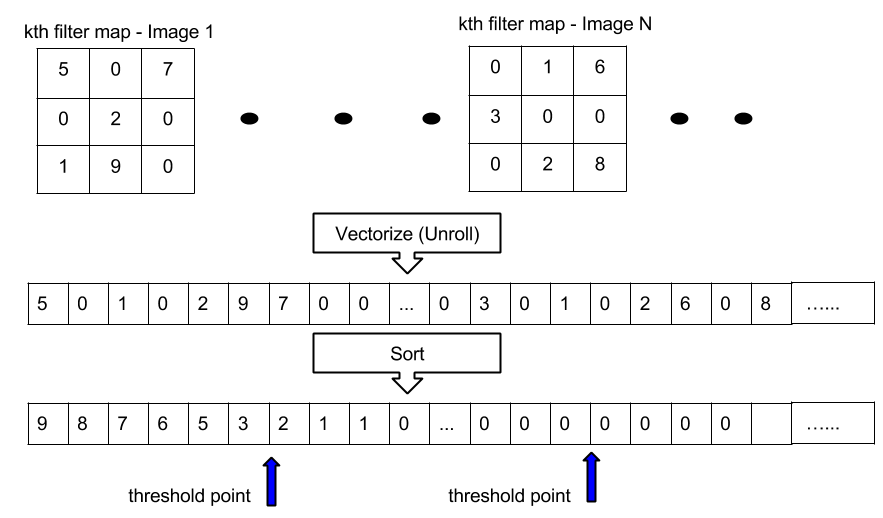
\includegraphics[scale=0.15]{images/vectorize.png}
\caption{Illustration of the procedure for computing filter entropy.}
\label{fig:vectorize}
\end{figure}

We use Area under this entropy curve (AuE) to quantify selectivity of each filter. The distribution of AuE for all filters across the seven layers of the CNN is illustrated in fig \ref{fig:fine-hist}. Next, in order to determine the overall change in a layer's tuning we use the Mean Cumulative AuE (MC-AuE) of filters sorted in decreasing order of their individual AuE's. Fig \ref{fig:fine-entropy} plots MC-AuE as a function of fraction of filters in each layer. 

\begin{figure}[H]
\centering
\subfloat{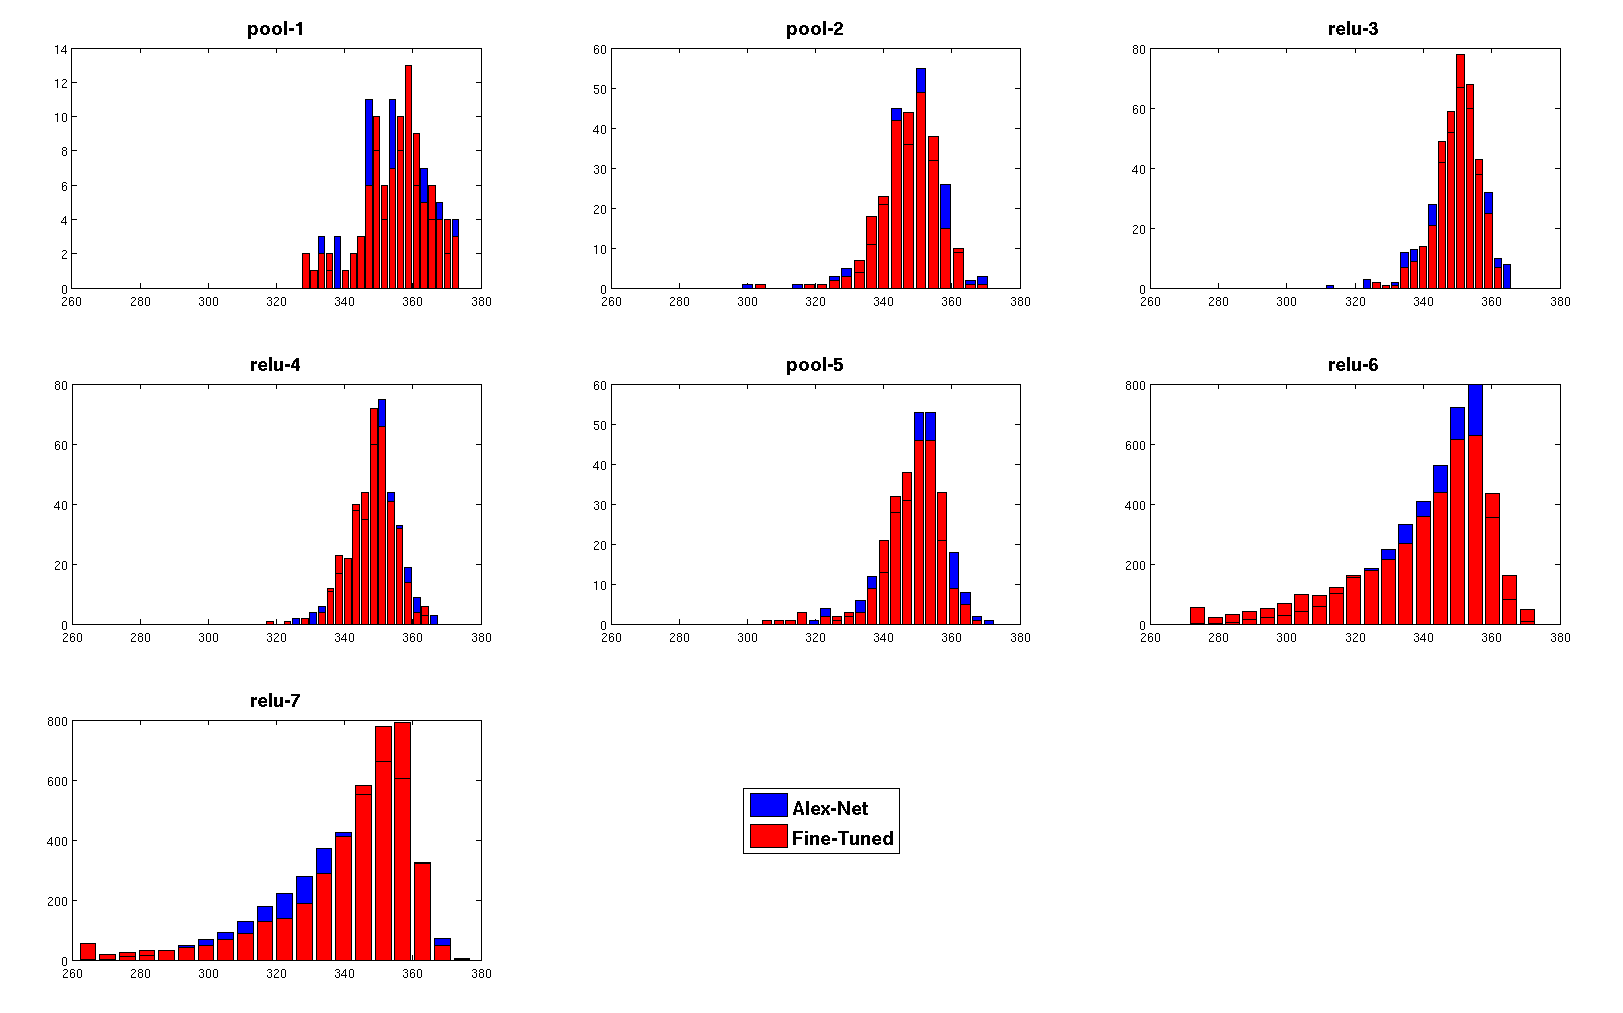
\includegraphics[height=6.5cm]{images/ent_hist.png}}
\caption{Distribution of AuE for different layers in Alex-Net and FT-Net. X-axis is the entropy and the Y-axis is the number of filters. Notice that the left tail for relu 6 and 7 becomes heavier after finetuning.}
\label{fig:fine-hist}
\end{figure}

\begin{figure}
\centering
\subfloat{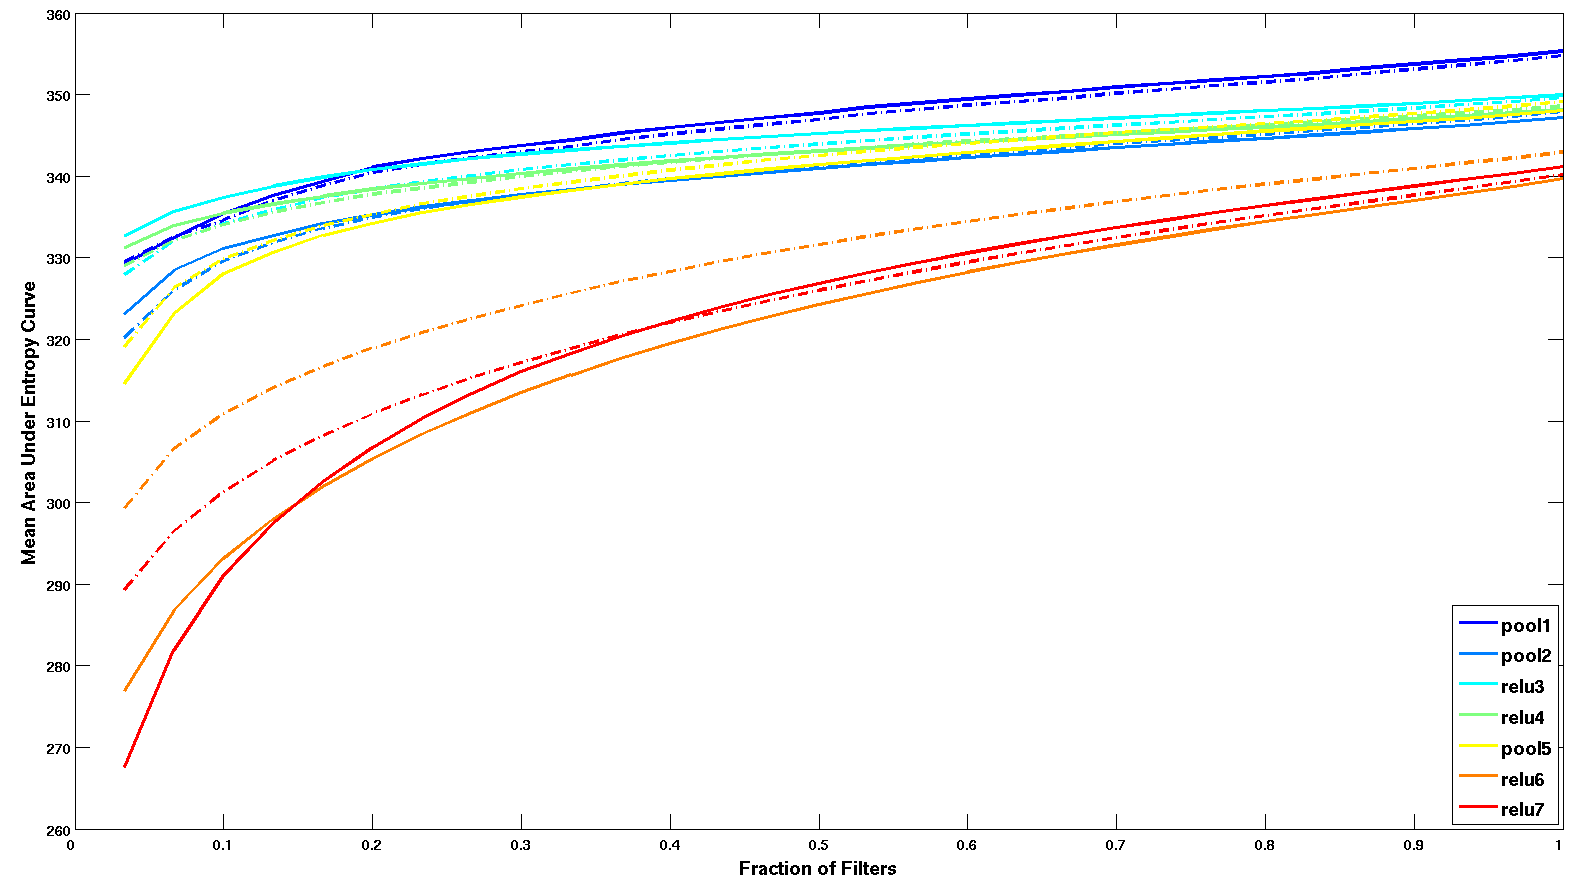
\includegraphics[scale=0.15]{images/entropy_variation.png}}
\caption{Mean Cumulative AuE plotted as fraction of filters (see sec \ref{sub:fine-entropy}). (Dash-Dot Line :Alex-Net, Solid Line: Fine-Tuned Network).}
\label{fig:fine-entropy}
\end{figure}

From this analysis we draw 2 conclusions. The first that although the entropy of filters decreases, the change in entropy between layer 1 and layer 5 is small as compared to the change which happens while going from layer 5 to layer 6. Second, finetuning mostly reduces the entropy of filters in the fully connected layers, there are small changes in layer 5 and negligible changes in other layers. Classification accuracy (measured as mAP) for GT-BBOX is detailed in \ref{table:gt-bbox-fine} is in agreement with our conclusions.

\setlength{\tabcolsep}{4pt}
\begin{table}
\begin{center}
\caption{mAP for gt-bbox classification(FT: Fine-Tuned,A-Net: Alex-Net).}
\label{table:gt-bbox-fine}
\begin{tabular}{ccc|ccc|ccc|ccc}
\hline\noalign{\smallskip}
Layer & A-Net & FT & Layer & A-Net & FT & Layer & A-Net & FT & Layer & A-Net & FT \\
\noalign{\smallskip}
\hline
\noalign{\smallskip}
pool-1 & 43.2 & 43.2  & relu-3 & 73.3 & 73.7 & pool-5 & 79.1 & 82.2 & relu-7 & 84.0 & 87.1 \\
pool-2  & 67.1 & 67.7 & relu-4 & 75.5 & 77.8 & relu-6 & 83.4 & 85.4 \\
\hline
\end{tabular}
\end{center}
\end{table}
\setlength{\tabcolsep}{1.4pt}

\subsection{Is finetuning only the fully-connected layers sufficient?}
\label{sub:fine-fc-only}
The observations made in \ref{sub:fine-entropy} indicate that finetuning the convolutional layers in the CNN may not be critical for achieving good-performance on novel datasets. We test this hypothesis on the 2 challenging tasks of object detection(PASCAL) and scene classification (SUN-397) by comparing the performance of a fully finetuned network with a network finetuned by only updating weights in the fully-connected (fc) layers. Our results are summarized in table \ref{table:fine-effect}.

\setlength{\tabcolsep}{2pt}
\begin{table}
\begin{center}
\caption{Comparison in performance on 4 tasks for 3 network models. (ft-net: finetuned, fc-ft: finetuning fc layers only). For PASCAL tasks we report the mAP and classification accuracy for SUN.}
\label{table:fine-effect}
\scalebox{0.85}{
\begin{tabular}{l|ccc|ccc|ccc|ccc}
\hline\noalign{\smallskip}
Layer & \multicolumn{3}{c}{img classification}  & \multicolumn{3}{c}{gt-bbox classification} & \multicolumn{3}{c}{detection} & \multicolumn{3}{c}{sun-397} \\
\hline
      & alex-net & ft-net & fc-ft & alex-net & ft-net & fc-ft & alex-net & ft-net & fc-ft  & alex-net & ft-net & fc-ft\\
\hline
pool-5   & 65.6 & 64.6 & - & 79.1 & 82.2 & 79.1  & 45.0 & 47.6 & 45.0 & - & - & - \\
relu-6   & 70.6 & 71.7 & - & 83.4 & 85.4 & 82.0  &  -   & 53.1 & 51.0 & - & - & -  \\
relu-7   & 73.6 & 73.2 & - & 84.0 & 87.1 & 83.4  & 45.5 & 54.1 & 53.3 & 53.1 & 56.1 & 55.5  \\
\hline
\end{tabular}}
\end{center}
\end{table}
\setlength{\tabcolsep}{1.4pt}

We find that indeed it is the case that the final performace in the detection setup only drops by 0.8 points and by 0.6 points for scene-classification. It is note-worthy that image classification accuracy on PASCAL is almost untouched by finetuning. This is suggestive of the fact finetuning is a task specific operation and finetuning for detection doesnot necessarily leads to an increase in classification performance, even though the classes and images are shared across PASCAL classification and detection challenges. 
It is also notable that although ft-net achieve superior performance on gt-bbox classification whereas the fc-ft fails to do so. We conjecture, that this is a consequence of the fact that for good performance on detection it is more critical to discriminate against background rather than to discriminate between classes on which both the networks are already doing a pretty good job. 

\setlength{\tabcolsep}{1pt}
\begin{table}
\begin{center}
\caption{Evaluation of effect finetuning towards the task of object detection. (l5, l6, l7: layers 5, 6 and 7 of Alex Net)}
\label{table:det-fine}
\scalebox{0.75}{
\begin{tabular}{l|cccccccccccccccccccc||c}
\hline\noalign{\smallskip}
layer & aero & bike & bird & boat & bottle & bus & car & cat & chair & cow & table & dog & horse & mbike & person & plant & sheep & sofa & train & tv & mAP \\
\noalign{\smallskip}
\hline
l5 & 51.9 & 61.1 & 36.8 & 28.4 & 23.7 & 52.3 & 60.8 & 48.4 & 24.9 & 47.1 & 47.5 & 42.1 & 55.6 & 58.7 & 42.5 & 24.5 & 46.9 & 39.3 & 52.0 & 55.4 & 45.0 \\
l5-ft & 57.8 & 63.9 & 38.8 & 28.0 & 29.0&54.8&66.9&51.3 & 30.5 & 52.1 & 45.2 & 43.2 & 57.3 & 58.8 & 46.0 & 27.2 & 51.2 & 39.3 & 53.3 & 56.6 & 47.6 \\
\hline 
l6-ft &63.5 & 66.3 & 48.7 & 38.1 & 30.6 & 61.4 & 70.9 & 60.3 & 34.8 & 57.8 & 47.6 & 53.6 & 59.8 & 63.5 & 52.5 & 29.8 & 54.6 & 48.2 & 58.5 & 62.2 & 53.1 \\
l6-fc-ft& 61.4 & 63.9 & 44.2 & 36.2 & 29.0 & 59.9 & 66.0 & 55.3 & 31.1 & 57.6 & 49.5 & 49.4 & 59.4 & 63.7 & 50.8 & 29.5 & 54.1 & 43.2 & 57.4 & 58.8 & 51.0 \\
\hline
l7 & 57.6 & 57.2 & 41.4 & 31.2 & 25.6 & 52.4 & 58.8 & 50.9 & 25.2 & 50.4 & 42.7 & 47.1 & 52.2 & 55.6 & 44.5 & 23.9 & 48.0 & 38.1 & 51.5 & 56.6 & 45.5 \\
l7-ft & 64.3 & 69.6 & 50.1 & 41.8 & 32.0 & 62.6 & 71.0 & 60.6 & 32.8 & 58.5 & 46.4 & 56.0 & 60.0 & 66.9 & 54.2 & 31.5 & 52.7 & 48.8 & 57.7 & 64.7 & 54.1 \\
l7-fc-ft & 62.9 & 65.2 & 47.5 & 39.0 & 30.3 & 63.1 & 68.4 & 59.7 & 34.2 & 58.5 & 52.0 & 53.8 & 60.7 & 65.3 & 53.0 & 30.2 & 55.5 & 46.3 & 57.7 & 62.2 & 53.3 \\
\hline
\end{tabular}}
\end{center}
\end{table}
\setlength{\tabcolsep}{1.4pt}

Detection performance obtained after using features from layers 5,6,7 for all pascal categories and the 3 network configurations is presented in table \ref{table:det-fine}. Notice that for both the finetuned networks there is big jump in the performance while going from layer 5 to 6 and a rather small jump from layer 6 to 7. For Alex-Net, the performance is virtually the same for layers 5 and 7. It is also notable, that although the performance for FT-net is better by 2.6 points at layer 5 - the performance is virtually the same at layer 7. (This indicates generic nature of pool-5 ? - **To-Do**)

\subsection{Discussion}
\label{sub:fine-discussion}
**To Do: Contrast to mid-level patches idea - where greedily select filters based on entropy
**To Do: Talk about Features being generic in layers 1-4 somewhat in 5 and that tuning of fc layers is most critical **


\section{Where is the information - location or magnitude?}
\label{sec-where-info}
The success of convolutional networks on a variety of vision tasks indicate that they are here to stay. In the computer vision literature the dominant models can be broadly grouped into 2 classes - namely BOW style approaches or template based scanning window search. Currently, it is unclear if we could use conv-nets features as building blocks for such systems or if completeley new ways of thinking about them is necessary. 
Instead of trying to provide a pre-mature answer to this question, we analyse how information is encoded across different layers of such  networks. We hope this analysis will serve as a starting point

. In this section we focus on answering the following two questions:
\begin{itemize}
\item How important is the location where a filter fires?
\item How much information is contained in the magnitude of filter activations?
\end{itemize}

We answer these questions using a set of carefully designed ablation studies. The difference between the baseline performance obtained by using vectorized  layer (i.e. i.e. "unrolling" a 3-dimensional layer of size $sz \times sz \times nf$ into a 1 dimensional vector) and an ablated feature vector is used as a measure of importance for factors under study. In all our experiments in this section, we train linear svms for evaluation.

\begin{figure}[H]
\centering
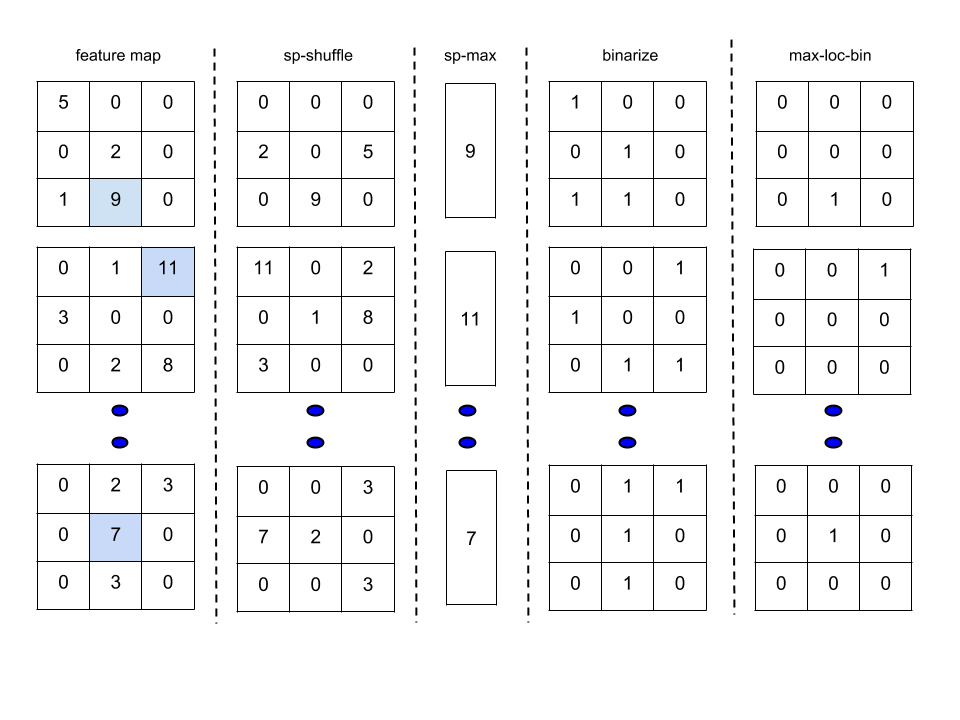
\includegraphics[height=6.5cm]{images/features.png}
\caption{Different feature ablations used in analysis described in sec. \ref{sub:imp-loc}, \ref{sub:imp-mag}. For the purpose of illustration, consider each 3*3 block in first column as a feature map. The second column shows \textit{spatial-shuffle}, i.e. the  result of applying an independent spatial random permutation to each feature map. Third column depicts \textit{spatial max}, i.e. selecting the max activation in each featue map. Fourth column illustrates \textit{binarization} whereas the last column selects the maximum value in each feature map, binarizes it but also retains the location where the filter fired.}
\label{fig:features}
\end{figure}

\subsection{How important is where a filter activates?}
\label{sub:imp-loc}
In order to understand the importance of location of firing of filter, we first use the spatial-shuffle feature transformation (see \ref{fig:features}) in which for each image and each feature map we use an independent random permutation to swap spatial locations. Note, we donot permute the filter activations across different filters - but for each filter we independently permute the spatial location. Such a feature transformation makes it almost impossible to learn anything about the spatial pattern of filter activations. Surprisingly, the performance only drops to 59.6 \% from 65.6 \% for Pool-5 on the task of image classification (see \ref{table:class-loc-mag}). 

\setlength{\tabcolsep}{4pt}
\begin{table}
\begin{center}
\caption{Mean AP on PASCAL-VOC 2007 Classification using various ablations as described in \ref{sub:imp-loc} -\ref{sub:imp-mag}.}
\label{table:class-loc-mag}
\begin{tabular}{lccccc}
\hline\noalign{\smallskip}
Layer Name & Unroll & Spatial-Shuffle & Spatial-Max & Binarize & Binarize+Loc\\
\noalign{\smallskip}
\hline
\noalign{\smallskip}
pool-1 & 25.1 & 15.0 & 19.5 & 25.4 \\
pool-2 & 44.9 & 33.5 & 40.2 & 43.0\\
conv-3 & 50.1 & 40.4 & 54.2 & 47.0\\
conv-4 & 54.2 & 45.3 & 57.0 & 51.3\\
pool-5 & 65.6 & 59.6 & 62.6 & 60.5\\
relu-6 & 70.6 &  -   &  -   & 71.4 \\
relu-7 & 73.6 &  -   &  -   & 74.1 \\
\hline
\end{tabular}
\end{center}
\end{table}
\setlength{\tabcolsep}{1.4pt}


To further probe this in our next experiment, we collapse the features of each layer by preserving only the maximum value for each filter. On classification this transformation does almost as good as the unrolled feature vector. But, for the task of detection this is brutal and the performance drops to 25.4 \% from 47.5 \% at the pool-5 level. Aprioiri this indicates it is important to consider where the filter fires for localization but for classification this is doesnot seems to be important. 

\setlength{\tabcolsep}{1pt}
\begin{table}
\begin{center}
\caption{Detection: Effect of various feature ablations using the R-CNN setup as described in ...}
\label{table:headings}
\tiny
\begin{tabular}{l|cccccccccccccccccccc||c}
\hline\noalign{\smallskip}
Feature & aero & bike & bird & boat & bottle & bus & car & cat & chair & cow & table & dog & horse & mbike & person & plant & sheep & sofa & train & tv & mAP \\
\noalign{\smallskip}
\hline
spMax & 35.0 & 38.7 & 17.3 & 16.9 & 13.9 & 38.4 & 45.6 & 29.2 & 11.0 & 20.2 & 21.0 & 23.5 & 27.2 & 37.0 & 20.5 & 7.0 & 30.3 & 13.4 & 28.3 & 32.9 & 25.4 \\
sm-bn-lc & 49.1 & 48.0 & 19.0 & 15.2 & 12.9 & 44.7 & 57.0 & 32.8 & 11.9 & 32.5 & 19.0 & 25.0 & 37.5 & 41.6 & 34.8 & 15.6 & 34.1 & 13.0 & 35.7 & 44.9 & 31.2 \\
crop-1 & 48.2 & 59.8 & 32.2 & 20.0 & 24.6 & 46.2 & 61.2 & 41.6 & 20.6 & 46.3 & 32.9 & 38.6 & 49.9 & 53.1 & 41.8 & 25.1 & 45.0 & 23.8 & 46.2 & 51.7 & 40.4 \\
binary & 57.9 & 61.3 & 32.6 & 24.7 & 27.5 & 55.0 & 64.7 & 49.8 & 25.3 & 47.4 & 44.5 & 40.3 & 54.6 & 56.4 & 43.6 & 27.1 & 48.4 & 41.6 & 54.3 & 57.6 & 45.7 \\
pool-5  & 57.8 & 63.9 & 38.8 & 28.0 & 29.0 & 54.8 & 66.9 & 51.3 & 30.5 & 52.1 & 45.2 & 43.2 & 57.3 & 58.8 & 46.0 & 27.2 & 51.2 & 39.3 & 53.3 & 56.6 & 47.6 \\
\noalign{\smallskip}
\hline
\end{tabular}
\end{center}
\end{table}
\setlength{\tabcolsep}{1.4pt}

\subsection{How important is the magnitude of activation ?}
\label{sub:imp-mag}
For answering this question, we binarize the feature vectors. Surprisingly this has little effect on detection. Also, the performance of fully-connected layers on the task of image classification is virtually un-affected. For other layers, the drop in performance is slightly larger as compared to taking the \textit{spatial max}. It is interesting to note that magnitude of the activations are more important for classification than for detection while the reverse seems to be true for detection. 

\subsection{Discussion}
** To Come ** 

\section{How common are Grand-Mother like Units ?}
\label{sec:grand-mother}
How information is represented in deep architectures such as convolutional neural networks is an open question. We know that the first layer ends up learning gabor like edge detectors and that units in the final layers are very class specific. However, we are far from understanding the representations learned in the middle layers. Developing this understanding is crucial in order to effectively devise methods capable of fully exploiting the rich feature hierarchy provided by convolutional networks.
Some recent work addressing this question has focussed on developing visualization techniques (zeiler, simoyan, google paper) to understand feature tuning of different filters. \cite{zeiler} presented a deconvolution strategy which effectively uses backprojection to find image regions which cause a particular filter to activate.  \cite{simoyan} on the other hand pose tuning as an optimization problem and try to estimate optimal stimuli for a given unit in the higher layers. \cite{google} train a massive non-convolutional network and show the presence of cat and people specific units learnt by their network. We feel that although visualizations are helpful they donot convey the full story. More-over they are subjective and it is unclear what conclusions one might draw. In particular, finding a few units tuned to people or cats tells us very little about what other units might be doing. To best of our knowledge there is no work which tries to objectively answer this question.

Also, most of such work can be treated as different interpretations of estimating/understanding P(Activation of a single unit | Class). Although this is linked to P(Class | Activation) via Bayes theorem it is hard to emperically estimate P(Class). More often than not our goal is to use to features for task of prediction. With this motivation we believe that P(Class | Activation) is also an important metric to study. One more way of looking at these metrics is the whether we are more interested to probe invariance of a particular filter or we are interested in understanding the discriminative power which it provides. A filter can be both highly invariant and very discrminative or higly invariant and very generic.  

**Information theoretic arguments ?? ** 

Aprioiri it is unclear whether discriminative information about a certain class is encoded in distribution of a group of filter activations or whether there are specific units tuned to specific classes. From the principles of efficient coding (such as Hoffman encoding) - an optimal code (Redundancy vs ...)

The question we pose is whether the representation learned by a deep conv-net consist of many "grand-mother cells" (specifically tuned units for various classes) or whether it is necessary to consider the distribution of activations across many filters to infer any semantics about the image. We develop two methods presented in the following subsections in an attempt to objectively answer this question.


A lot of recent (...) has focussed on understanding the invariance properties of each filter. In particular, in one form or the other they have focussed on estimating $P(Activation | Class)$. [simoyan and google] explicitly maximize this metric to find the optimal input for a unit. zeiler et al on the other hand start off with a specific image and use it for deconvolution. If a prioiri, we knew that information representation is not distributed and a very few neurons are necessary to represent a certain class - studying the invariance is the correct thing to do. However, if we believe that information is distributed - then we can have a group of filters wherein each filter by itself may not be tuned for a particular class but the activation of group of filters 

\subsection{Finding class specific units}
\label{sub:class-specific-unit}
In order to study the tuning properties of various units, for each PASCAL class we emperically estimate P(Class | Activation of unit > threshold) for all 256 filters in layer 5. For this purpose, we restrict ourselves to ground truth bounding boxes in contrast to full images as a single image may contain multiple objects and thereby confound any interpretations drawn from our analysis. 

Each filter in Pool-5 layer appears as $6 \times 6$ spatial map. Thus for each ground truth bounding box we get 36 activation samples for a particular unit. Given, N boxes we end up with 36N samples for each filter. For each filter, we sort the activations values and use this to compute the probability of a unit representing a class given its value is more than some threshold. We compute this probability for 1000 thr

From our analysis, we find that in order to predict the category of a given image, neither the magnitude nor the location of where filters activate is critical. On the other hand, 


As described in section .. we compute the entropy of each filter in the fifth layer of the network. Next, we rank all the filters by their entropy. At pool-5, each image produces a $6 \times 6 \times 256 $ feature vector (256 filter maps of size $6 \times 6$). For each filter map - we select the maximum activation which results into a 256-dimensional vector. Now, we train SVM 
 
For tasks of image classification, bounding box classification - position doesnot really matter. 

\subsection{How many units do we need?}
\label{sub:how-many}
The tuning analysis presented in section \ref{sub:class-specific-unit} is not sufficient by itself to answer how many units are needed in order to classify a given image. This is because, there might be important information in simultaneous firing of a group of filters which is ignored while looking only at individual filters. 

Consequently, in order to answer the above posed question we train linear a svm for each class using only a subset of 256 pool-5 filters. In particular we construct subsets of size k, where k takes the values - [1,2,3,5,10,15,20,25,30,35,40,45, \newline 50,80, 100,128,256]. A subset of size k is constucted independently for each class using a greedy selection strategy described in figure \ref{fig:sel-strategy}. We use the variation in performance with the number of filters needed as a metric to evaluate how many filters are needed for each class. 
  
\begin{figure}[H]
\centering
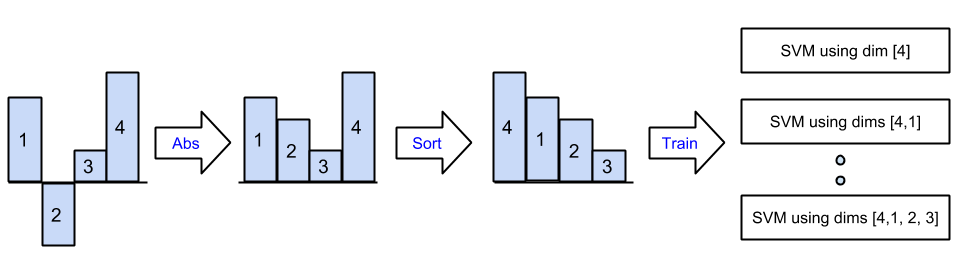
\includegraphics[scale=0.30]{images/how-many.png}
\caption{Illustration of our greedy strategy for constructing subsets of filters. For each class we first train a linear-svm using the spatial-max feature transformation described in section \ref{sub:imp-loc}. Spatial-max leaves us with a 256-D vector wherein each dimension has a one to one correspondence with 256 pool-5 filters. We use the magnitude of each dimension of the learnt weight vector as a proxy for the importance of that dimension towards discriminating a given class. For the purpose of illustration we describe the procedure with a 4-D weight vector shown on the extreme left (the numbers on each bar are the "dimension"). Firstly, we take the absolute value for each dimension and then sort the dimensions based on this value. Then, we chose the top k filters/dimensions from this ranked list to construct a subset of size k.}
\label{fig:sel-strategy}
\end{figure}

The results of our analysis are summarized in fig \ref{fig:svm-sel-dims} and table \ref{table:num-fil}. For classes such as persons, cars, cats we require a relatively few number of filters, but for most of the classes we need to look at around 30-40 filters to achieve atleast 90\% of the full performance. This also indicates, that for a few classes yes, there are grand-mother kind of neurons but for a lot of classes the representation is distributed. Also, as expected the fine-tuned network requires activations of a fewer numbers of filters to achieve the same performance but this reduction in number of filters is not large. 

\begin{figure}[H]
\centering
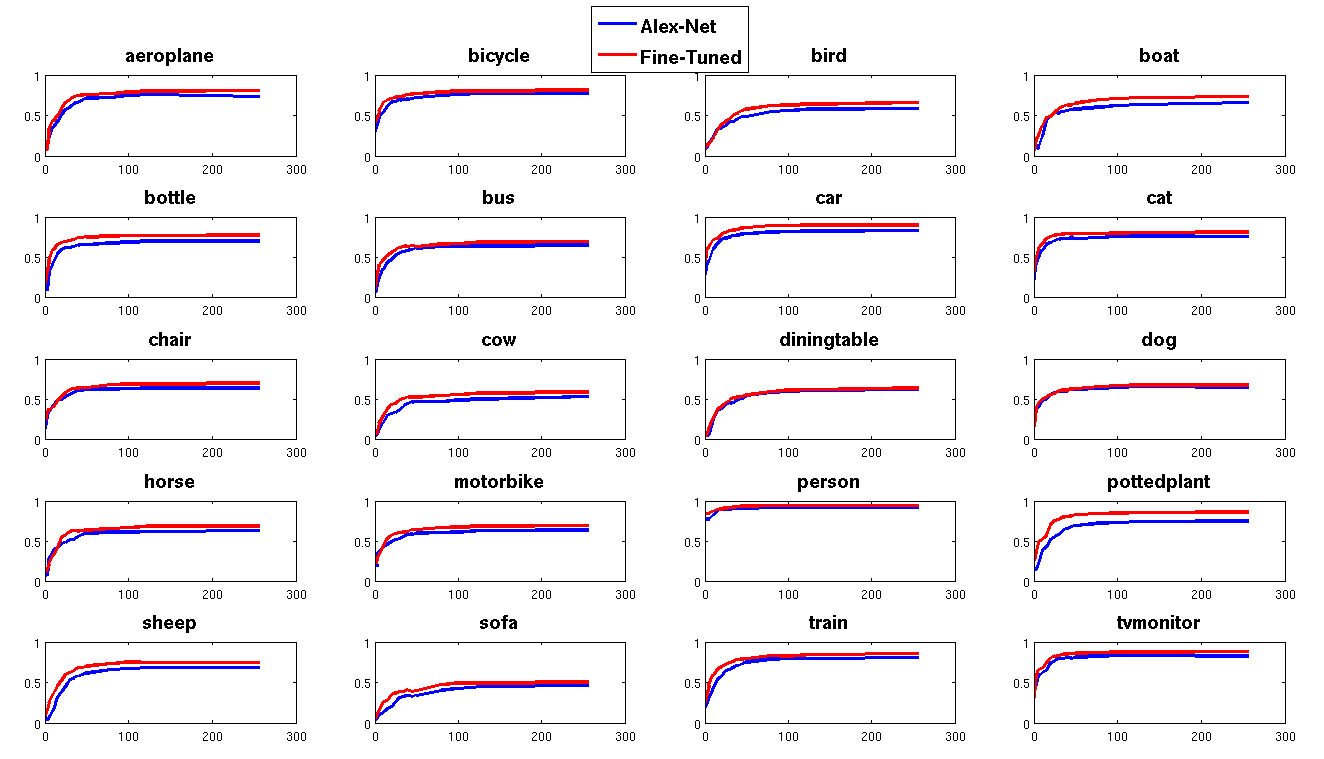
\includegraphics[height=6.5cm]{images/svm_seldims.png}
\caption{Analysis of how many filters are required to classify ground truth bounding boxes for 20 categories taken from PASCAL-2007 detection challenge. The y-axis in each of plot represents classification accuracy measured as mean-ap where as x-axis stand for the number of filters.)}
\label{fig:svm-sel-dims}
\end{figure}



\setlength{\tabcolsep}{1pt}
\begin{table}
\begin{center}
\caption{Number of filters required to achieve 50\% ,90\% of the full performance for PASCAL classes using Alex-Net(AN) and the Fine-Tuned network(FT)}
\label{table:num-fil}
\tiny
\begin{tabular}{lc||cccccccccccccccccccc}
\hline\noalign{\smallskip}
Net & AP & aero & bike & bird & boat & bottle & bus & car & cat & chair & cow & table & dog & horse & mbike & person & plant & sheep & sofa & train & tv \\
\noalign{\smallskip}
\hline
AN & 50 & 15 & 3 & 15 & 15 & 10 & 10 & 3 & 2 & 5 & 15 & 15 & 2 & 10 & 3 & 1 & 10 & 20 & 25 & 10 & 2 \\ 
FT & 50 & 10 & 1 & 20 & 15 & 5 & 5 & 2 & 2 & 3 & 10 & 15 & 3 & 15 & 10 & 1 & 5 & 15 & 15 & 5 & 2 \\
\hline
\noalign{\smallskip}
AN & 90 & 40 & 35 & 80 & 80 & 35 & 40 & 30 & 20 & 35 & 100 & 80 & 30 & 45 & 40 & 15 & 45 & 50 & 100 & 45 & 25 \\
FT & 90 & 35 & 30 & 80 & 80 & 30 & 35 & 25 & 20 & 35 & 50 & 80 & 35 & 30 & 40 & 10 & 35 & 40 & 80 & 40 & 20 \\
\hline
\end{tabular}
\end{center}
\end{table}
\setlength{\tabcolsep}{1.4pt}


\section{How do the different layers of a CNN train over time?}
\label{sec:speed}
Convolutional neural networks take a long time to train. For achieving state of art accuracy on the imagenet challenge these networks are often trained on high-end GPUs for more than 7 days. Even our implementation of fine-tuning following the approach proposed in \cite{Rcnn} takes more than 12 hours on a Nvidia Tesla-K40. Any speeds up in training will allow for a rich exploration of network architectures and parameters which is currently not possible.    

As a first step towards addressing this problem, we looked at the evolution of training loss and validation accuracy as the training progresses (fig \ref{fig:conv1}.) The top-1 accuracy on the imagenet validation set at 15K iterations is at 29.5 \% and 38.13\% at 50K iterations (compared to 57.4 \% at 310K iterations). The training loss rapidly increases initially and then there is a slow sluggish decay except at the stage where learning rate is decimated by a factor of 10 at 100K iterations.

\begin{figure}
\centering
\subfloat{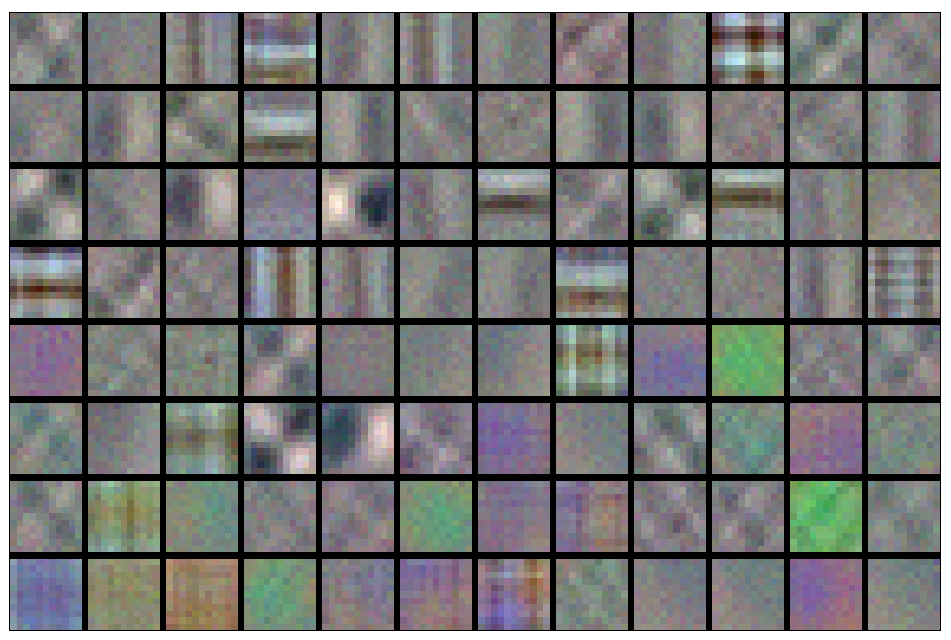
\includegraphics[scale=0.10]{images/l1_filters_iter5000.png}} \hspace{2mm}
\subfloat{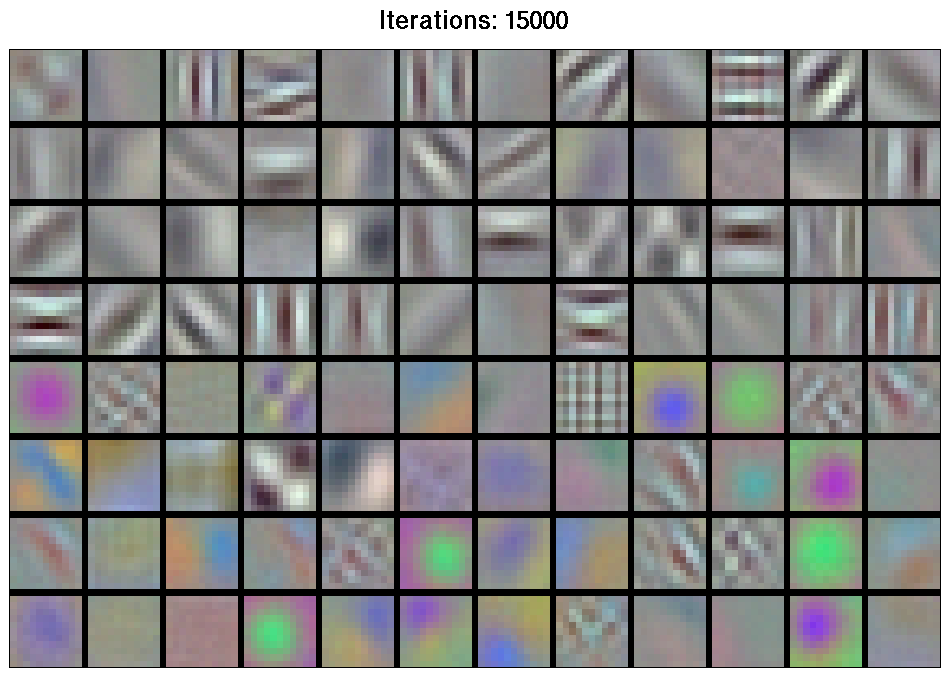
\includegraphics[scale=0.10]{images/l1_filters_iter15000.png}} \hspace{2mm}
\subfloat{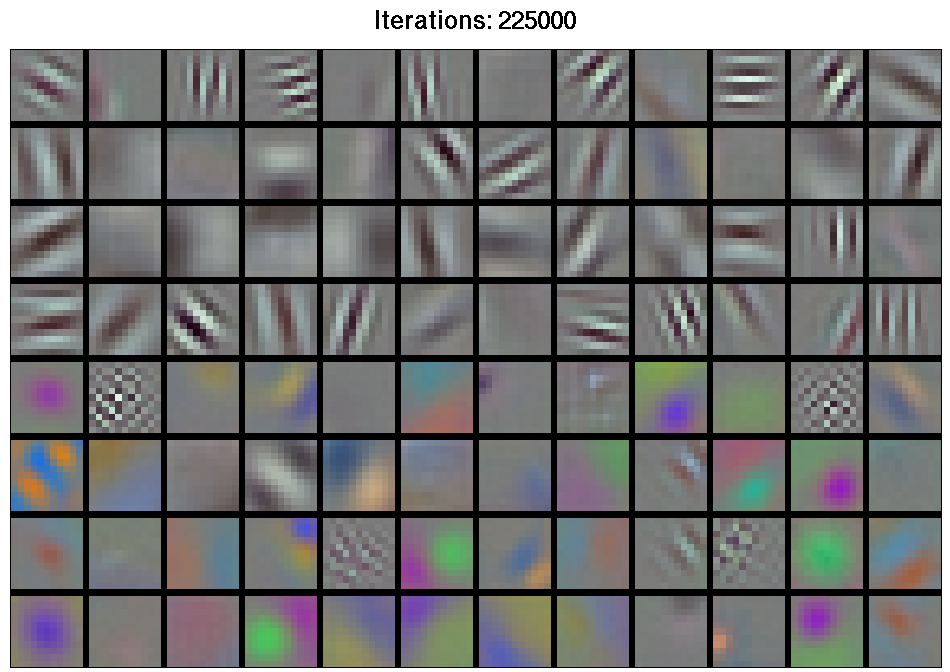
\includegraphics[scale=0.10]{images/l1_filters_iter225000.png}} \\
\subfloat{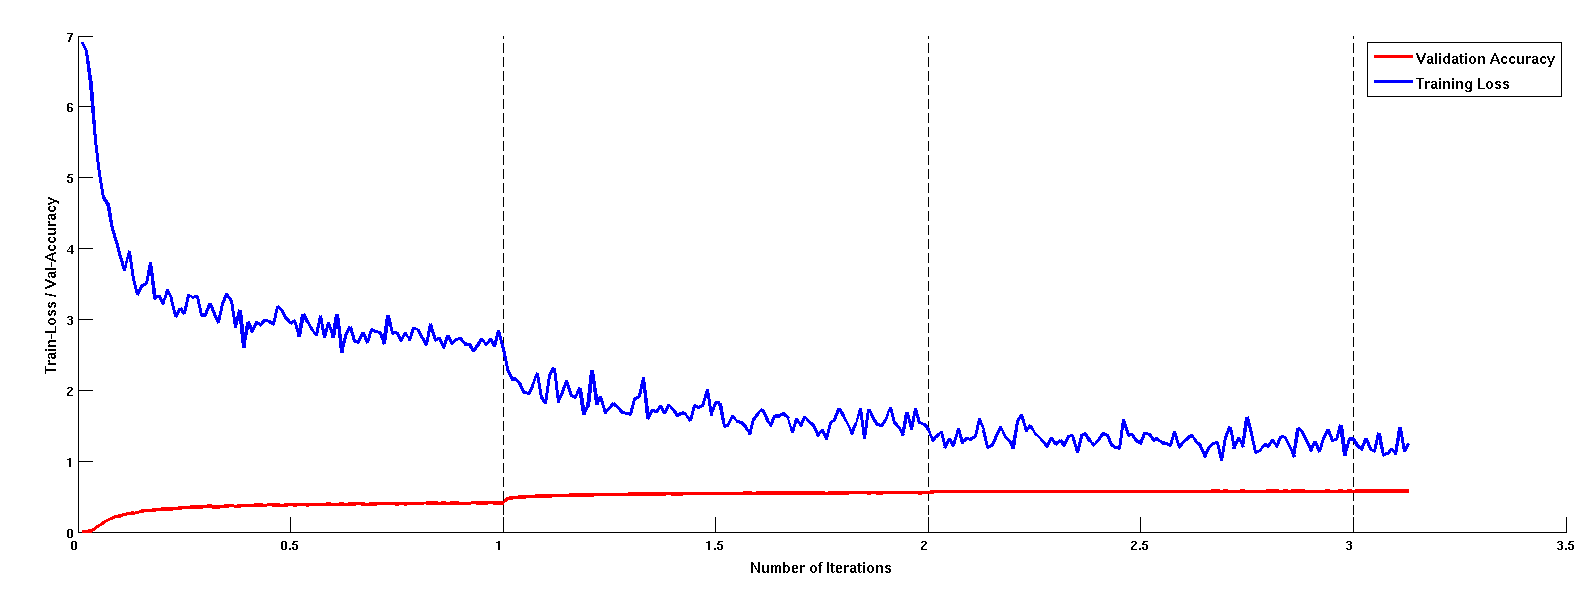
\includegraphics[scale=0.15]{images/training_loss.png}}
\caption{The first row shows conv-1 filters at 5K, 15K and 225K training iteration. The second row shows the evolution of training loss and top-1 accuracy on imagenet ilsvrc-2012 validation set as a function of number of iterations.}
\label{fig:conv1}
\end{figure}

The first question we ask is - Is there is an insightful intepretation of the fast intial drop in training loss? Towards this end, we visualized layer 1 filters at different time instances. Surprisingly, we found that within 15K iterations these filters look almost identical to what they would be by the end of the training (See fig \ref{fig:conv1}). This naturally leads us to ask the following questions:
\begin{itemize}
\item {How fast do different layers train? }
\item {Given that discriminative pre-training is helpful, is it the case that there exists a critical point after which learning on imagenet is not helpful for generalizing to other datasets/tasks? A "yes" answer to this question would imply that we can indeed speed-up finetuning.}
\end{itemize}  

For a better understanding. we evaluated performance of a linear svm classifier learned on features extracted from individual layers on Pascal 2007 classification challenge. The results are summarized in table \ref{table:det-traj-classify}.It is quite surprising to note that by 15K iterations all layers are within 80\% and at 50K iterations within 90\% of there final performance. This strongly indicates that a great portion of training required for generalization happens quite quickly. 

\setlength{\tabcolsep}{4pt}
\begin{table}
\begin{center}
\caption{Variation in classification accuracy (mean-AP) on PASCAL VOC 2007 challenge using features extracted from different layers of Alex-Net as a function of number of iterations.}
\label{table:det-traj-classify}
\begin{tabular}{lcccccccc}
\hline\noalign{\smallskip}
Layer  & 5K & 15K & 25K & 35K & 45K & 95K & 105K & 310K \\
\noalign{\smallskip}
\hline
\noalign{\smallskip}
pool-1 & 23.0 & 24.3 & 24.4 & 24.5 & 24.6 & 24.8 & 24.7 & 25.1\\
pool-2 & 33.7 & 40.4 & 40.9 & 41.8 & 42.0 & 43.2 & 44.0 & 45.0\\
conv-3 & 34.2 & 46.8 & 47.0 & 48.2 & 48.5 & 49.4 & 51.6 & 50.1\\
conv-4 & 33.5 & 49.0 & 48.7 & 50.2 & 50.6 & 51.6 & 54.1 & 54.2\\
pool-5 & 33.0 & 53.4 & 55.0 & 56.8 & 57.4 & 59.2 & 63.5 & 65.6\\
relu-6 & 34.2 & 59.7 & 62.6 & 62.7 & 64.1 & 65.6 & 69.3 & 70.6\\
relu-7 & 30.9 & 61.3 & 64.1 & 65.1 & 65.8 & 67.8 & 71.8 & 73.2\\
\hline
\end{tabular}
\end{center}
\end{table}
\setlength{\tabcolsep}{1.4pt}

Motivated by these observations we trained a 50-50 network (50K iterations on imagenet and finetuned for 50K iterations using the procedure described in sec. \ref{sub:fine-train}) and evaluated its performance on the  Pascal 2007 detection challenge (see table \ref{table:det-trajectory} for results). Consistent with our earlier results we find that this network achieves a surprising performance of 48.6 mean AP points compared to 54.1 achieved by pre-training for 310K iterations. 

\setlength{\tabcolsep}{1pt}
\begin{table}
\begin{center}
\caption{Performance of 50-50 network for detection on pascal-voc-2007 challenge. (l5 is pool-5 and l7 is relu-7)}
\label{table:det-trajectory}
\scalebox{0.70}{
\begin{tabular}{l|cccccccccccccccccccc||c}
\hline\noalign{\smallskip}
Feature & aero & bike & bird & boat & bottle & bus & car & cat & chair & cow & table & dog & horse & mbike & person & plant & sheep & sofa & train & tv & mAP \\
\noalign{\smallskip}
\hline
l5(50-50) & 55.2 & 58.4 & 31.0 & 28.8 & 21.0 & 53.5 & 63.6 & 41.0 & 25.4 & 44.7 & 40.9 & 34.9 & 49.5 & 56.9 & 43.8 & 25.2 & 45.3 & 31.2 & 48.7 & 54.4 & 42.7 \\
l5 (full) & 57.8 & 63.9 & 38.8 & 28.0 & 29.0&54.8&66.9&51.3 & 30.5 & 52.1 & 45.2 & 43.2 & 57.3 & 58.8 & 46.0 & 27.2 & 51.2 & 39.3 & 53.3 & 56.6 & 47.6 \\
\hline
l7(50-50) & 58.7 & 64.8 & 38.2 & 34.9 & 25.9 & 59.5 & 69.5 & 46.2 & 28.7 & 52.4 & 45.2 & 44.3 & 57.3 & 63.4 & 52.4 & 28.0 & 51.5 & 34.9 & 56.0 & 59.4 & 48.6 \\
l7(full) & 64.3 & 69.6 & 50.1 & 41.8 & 32.0 & 62.6 & 71.0 & 60.6 & 32.8 & 58.5 & 46.4 & 56.0 & 60.0 & 66.9 & 54.2 & 31.5 & 52.7 & 48.8 & 57.7 & 64.7 & 54.1 \\
\hline
\end{tabular}}
\end{center}
\end{table}
\setlength{\tabcolsep}{1.4pt}

The take home message from this analysis is that a majority of training happens very early on in the training and a lot of time is spent to achieve the final few points. (**Ross do we suggest any directions for reducing training time? **)

\section{Conclusions}
\label{sec:concl}
The paper ends with a conclusion. 

\clearpage\mbox{}Page \thepage\ of the manuscript.

\clearpage

\bibliographystyle{splncs}
\bibliography{egbib}
\end{document}
